\section{Testaufbau \& Ergebnisse}
\label{sec:test}

// TODO: erkläre hier den Testaufbau den wir gehabt haben und wie sich das Tool hier verhalten hat. Eventuell mit ein paar Screenshots mit Realdaten. Hier werden ein paar Seiten zusammenkommen weil wir vermutlich mehrere Tests durchführen (zb. so hat sich das System verhalten mit 3 angesteckten Geräten und so mit 20, ...)

\subsubsection{Testaufbau}
// Welche Switche sind wo? Welche Geräte auf welchen Ports angesteckt.

// Konfiguration vom Tool

\subsubsection{Testablauf}

// Erklärung wie das Ganze abgelaufen ist (Entweder Christopher oder Felix beschreiben das)

In Abbildung \ref{fig:portDetails} sieht man die Auswirkungen durch die Deaktivierung und anschließender Aktivierung eines Ports bezüglich der Werte die durch SNMP erhalten werden. Zwischen der 47 und 48 Messung im Abfragezeitraum wurde das Port per Administration deaktiviert. Augenblicklich fallen die Werte, die mit dem tatsächlichen Verbrauch des Gerätes auf diesen Port zu tun haben, auf 0. 

Bei oder kurz vor Messung 70 wurde das Port wieder aktiviert. Wie man sieht, stieg hierbei der Wert für \textit{PwrAllocated} kurzzeitig auf ein lokales Maximum. Dies liegt daran, dass der Port für den Einschaltvorgang des Gerätes, welches an dem Port hängt, eine höhere Leistung anbieten kann. Kurz darauf normalisiert sich dieser Wert wieder und fällt auf das Mittel (welches vom Switch berechnet wird) zurück.

Auch der tatsächliche Verbrauch steigt von Messung 70 beginnend an auf den Wert den er vor der Abschaltung gehabt hat. Diesen Zustand hat er nach circa 4 Messungen wieder erreicht.

\begin{figure}[h]
    \centering
    \leavevmode
    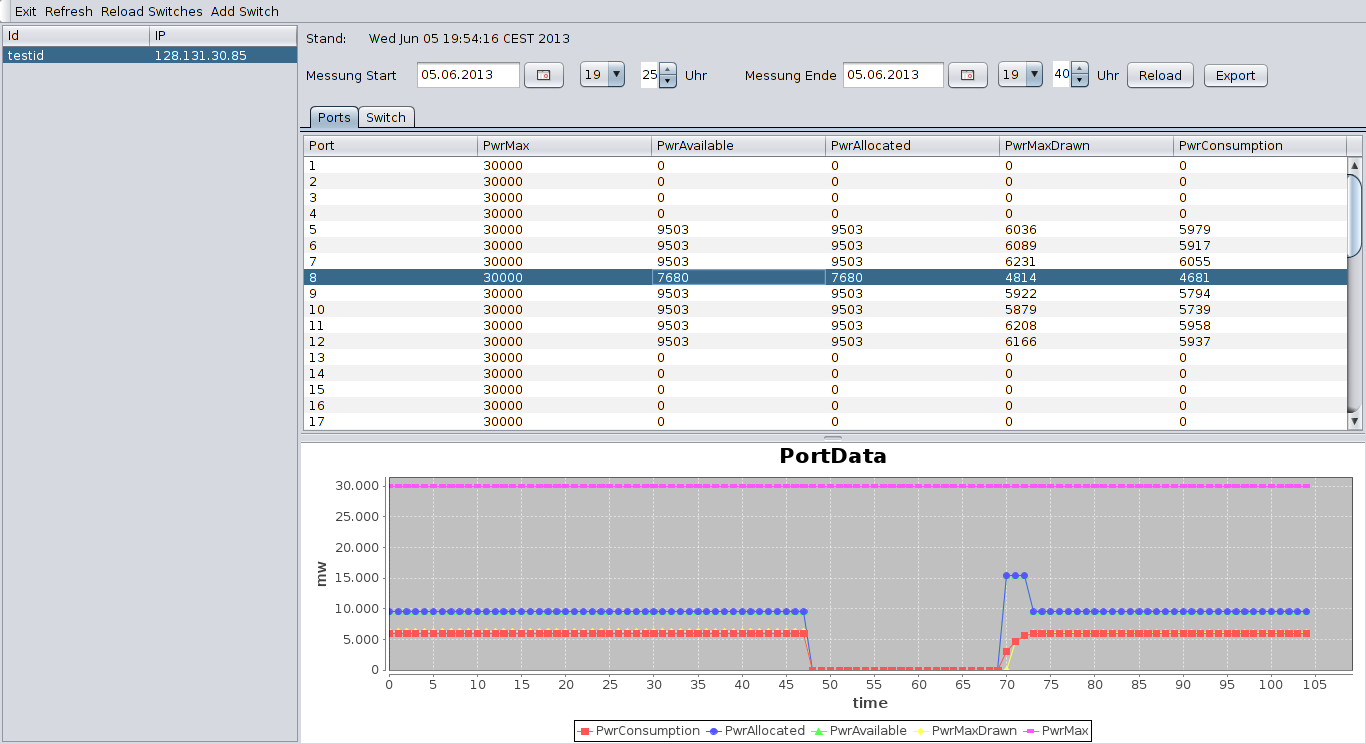
\includegraphics[width=1.0\linewidth]{figures/portDetails}
    \caption{Screenshot Verlauf Port Detail}
    \label{fig:portDetails}
\end{figure}

// Erkläre warum Grafik von Switch so aussieht wie sie aussieht
In Abbildung \ref{fig:switchDetails} sieht man die Auswirkungen durch die Deaktivierung und anschließender Aktivierung der Ports im definierten Testszenario.

\begin{figure}[h]
    \centering
    \leavevmode
    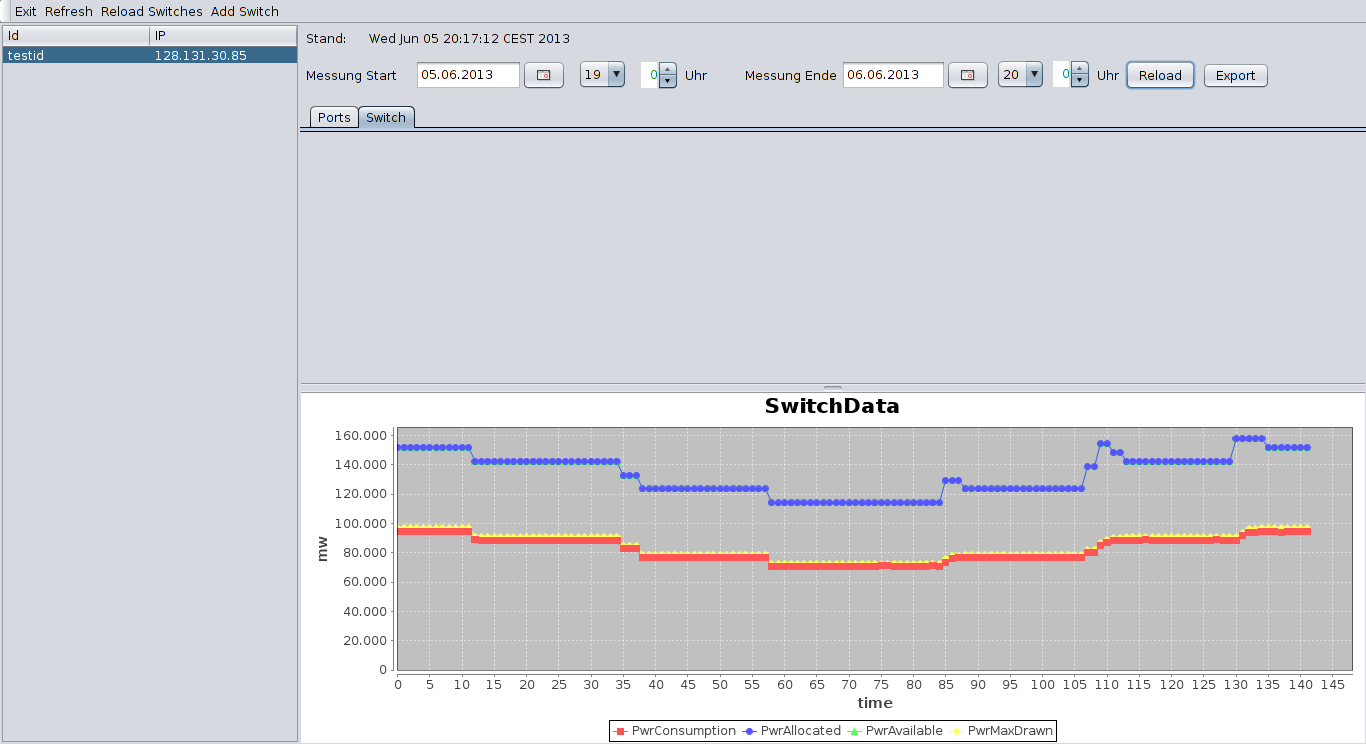
\includegraphics[width=1.0\linewidth]{figures/switchDetails}
    \caption{Screenshot Verlauf Switch Detail}
    \label{fig:switchDetails}
\end{figure}
